\documentclass[twoside]{book}

% Packages required by doxygen
\usepackage{fixltx2e}
\usepackage{calc}
\usepackage{doxygen}
\usepackage[export]{adjustbox} % also loads graphicx
\usepackage{graphicx}
\usepackage[utf8]{inputenc}
\usepackage{makeidx}
\usepackage{multicol}
\usepackage{multirow}
\PassOptionsToPackage{warn}{textcomp}
\usepackage{textcomp}
\usepackage[nointegrals]{wasysym}
\usepackage[table]{xcolor}

% Font selection
\usepackage[T1]{fontenc}
\usepackage[scaled=.90]{helvet}
\usepackage{courier}
\usepackage{amssymb}
\usepackage{sectsty}
\renewcommand{\familydefault}{\sfdefault}
\allsectionsfont{%
  \fontseries{bc}\selectfont%
  \color{darkgray}%
}
\renewcommand{\DoxyLabelFont}{%
  \fontseries{bc}\selectfont%
  \color{darkgray}%
}
\newcommand{\+}{\discretionary{\mbox{\scriptsize$\hookleftarrow$}}{}{}}

% Page & text layout
\usepackage{geometry}
\geometry{%
  a4paper,%
  top=2.5cm,%
  bottom=2.5cm,%
  left=2.5cm,%
  right=2.5cm%
}
\tolerance=750
\hfuzz=15pt
\hbadness=750
\setlength{\emergencystretch}{15pt}
\setlength{\parindent}{0cm}
\setlength{\parskip}{3ex plus 2ex minus 2ex}
\makeatletter
\renewcommand{\paragraph}{%
  \@startsection{paragraph}{4}{0ex}{-1.0ex}{1.0ex}{%
    \normalfont\normalsize\bfseries\SS@parafont%
  }%
}
\renewcommand{\subparagraph}{%
  \@startsection{subparagraph}{5}{0ex}{-1.0ex}{1.0ex}{%
    \normalfont\normalsize\bfseries\SS@subparafont%
  }%
}
\makeatother

% Headers & footers
\usepackage{fancyhdr}
\pagestyle{fancyplain}
\fancyhead[LE]{\fancyplain{}{\bfseries\thepage}}
\fancyhead[CE]{\fancyplain{}{}}
\fancyhead[RE]{\fancyplain{}{\bfseries\leftmark}}
\fancyhead[LO]{\fancyplain{}{\bfseries\rightmark}}
\fancyhead[CO]{\fancyplain{}{}}
\fancyhead[RO]{\fancyplain{}{\bfseries\thepage}}
\fancyfoot[LE]{\fancyplain{}{}}
\fancyfoot[CE]{\fancyplain{}{}}
\fancyfoot[RE]{\fancyplain{}{\bfseries\scriptsize Generated by Doxygen }}
\fancyfoot[LO]{\fancyplain{}{\bfseries\scriptsize Generated by Doxygen }}
\fancyfoot[CO]{\fancyplain{}{}}
\fancyfoot[RO]{\fancyplain{}{}}
\renewcommand{\footrulewidth}{0.4pt}
\renewcommand{\chaptermark}[1]{%
  \markboth{#1}{}%
}
\renewcommand{\sectionmark}[1]{%
  \markright{\thesection\ #1}%
}

% Indices & bibliography
\usepackage{natbib}
\usepackage[titles]{tocloft}
\setcounter{tocdepth}{3}
\setcounter{secnumdepth}{5}
\makeindex

% Hyperlinks (required, but should be loaded last)
\usepackage{ifpdf}
\ifpdf
  \usepackage[pdftex,pagebackref=true]{hyperref}
\else
  \usepackage[ps2pdf,pagebackref=true]{hyperref}
\fi
\hypersetup{%
  colorlinks=true,%
  linkcolor=blue,%
  citecolor=blue,%
  unicode%
}

% Custom commands
\newcommand{\clearemptydoublepage}{%
  \newpage{\pagestyle{empty}\cleardoublepage}%
}

\usepackage{caption}
\captionsetup{labelsep=space,justification=centering,font={bf},singlelinecheck=off,skip=4pt,position=top}

%===== C O N T E N T S =====

\begin{document}

% Titlepage & ToC
\hypersetup{pageanchor=false,
             bookmarksnumbered=true,
             pdfencoding=unicode
            }
\pagenumbering{roman}
\begin{titlepage}
\vspace*{7cm}
\begin{center}%
{\Large Control of Drones using Oculus Rift }\\
\vspace*{1cm}
{\large Generated by Doxygen 1.8.11}\\
\end{center}
\end{titlepage}
\clearemptydoublepage
\tableofcontents
\clearemptydoublepage
\pagenumbering{arabic}
\hypersetup{pageanchor=true}

%--- Begin generated contents ---
\chapter{Oculus Drift Package}
\label{index}\hypertarget{index}{}\begin{DoxyAuthor}{Author}
Lukasz Dracz 

Simone Mazzola 

Suraj Pattar
\end{DoxyAuthor}
\hypertarget{index_intro_sec}{}\section{Introduction}\label{index_intro_sec}
The Oculus Drift provides three control schemes for controlling a firefly asctec drone using an oculus rift and keyboard. The Oculus Drift consists of four nodes that can be run.

Oculus-\/drift republishes images from the firefly stereo camera to the oculus

Oculus-\/control provides the first control scheme using the Oculus orientation info

With this node it is possible to move into any position using the proper sequence of commands.

oculus-\/control-\/alternative provides a similar control scheme as oculus-\/control but limits

the oculus to the xy plane it is currently located and changes tilting in the z axis to movement

in the left or right of the robot.

oculus-\/control-\/keyboard allows the control of the firefly drone through keyboard commands in the

terminal (that needs to be active). 
\chapter{File Index}
\section{File List}
Here is a list of all files with brief descriptions\+:\begin{DoxyCompactList}
\item\contentsline{section}{/home/lukasz/zros/src/oculus-\/drift/src/\hyperlink{image-publisher_8cpp}{image-\/publisher.\+cpp} }{\pageref{image-publisher_8cpp}}{}
\item\contentsline{section}{/home/lukasz/zros/src/oculus-\/drift/src/\hyperlink{oculus-control-alternative_8cpp}{oculus-\/control-\/alternative.\+cpp} }{\pageref{oculus-control-alternative_8cpp}}{}
\item\contentsline{section}{/home/lukasz/zros/src/oculus-\/drift/src/\hyperlink{oculus-control-keyboard_8cpp}{oculus-\/control-\/keyboard.\+cpp} }{\pageref{oculus-control-keyboard_8cpp}}{}
\item\contentsline{section}{/home/lukasz/zros/src/oculus-\/drift/src/\hyperlink{oculus-control_8cpp}{oculus-\/control.\+cpp} }{\pageref{oculus-control_8cpp}}{}
\item\contentsline{section}{/home/lukasz/zros/src/oculus-\/drift/src/\hyperlink{oculus-drift_8cpp}{oculus-\/drift.\+cpp} }{\pageref{oculus-drift_8cpp}}{}
\end{DoxyCompactList}

\chapter{File Documentation}
\hypertarget{CMakeLists_8txt}{}\section{/home/lukasz/zros/src/oculus-\/drift/\+C\+Make\+Lists.txt File Reference}
\label{CMakeLists_8txt}\index{/home/lukasz/zros/src/oculus-\/drift/\+C\+Make\+Lists.\+txt@{/home/lukasz/zros/src/oculus-\/drift/\+C\+Make\+Lists.\+txt}}

\hypertarget{oculus-control-alternative_8cpp}{}\section{/home/lukasz/zros/src/oculus-\/drift/src/oculus-\/control-\/alternative.cpp File Reference}
\label{oculus-control-alternative_8cpp}\index{/home/lukasz/zros/src/oculus-\/drift/src/oculus-\/control-\/alternative.\+cpp@{/home/lukasz/zros/src/oculus-\/drift/src/oculus-\/control-\/alternative.\+cpp}}
{\ttfamily \#include $<$ros/console.\+h$>$}\\*
{\ttfamily \#include $<$tf/transform\+\_\+broadcaster.\+h$>$}\\*
{\ttfamily \#include \char`\"{}geometry\+\_\+msgs/\+Pose\+Stamped.\+h\char`\"{}}\\*
{\ttfamily \#include \char`\"{}geometry\+\_\+msgs/\+Quaternion.\+h\char`\"{}}\\*
{\ttfamily \#include $<$thread$>$}\\*
{\ttfamily \#include $<$chrono$>$}\\*
{\ttfamily \#include $<$signal.\+h$>$}\\*
{\ttfamily \#include $<$termios.\+h$>$}\\*
{\ttfamily \#include $<$stdio.\+h$>$}\\*
{\ttfamily \#include $<$Eigen/\+Core$>$}\\*
{\ttfamily \#include $<$mav\+\_\+msgs/conversions.\+h$>$}\\*
{\ttfamily \#include $<$mav\+\_\+msgs/default\+\_\+topics.\+h$>$}\\*
{\ttfamily \#include $<$ros/ros.\+h$>$}\\*
{\ttfamily \#include $<$std\+\_\+srvs/\+Empty.\+h$>$}\\*
{\ttfamily \#include $<$trajectory\+\_\+msgs/\+Multi\+D\+O\+F\+Joint\+Trajectory.\+h$>$}\\*
{\ttfamily \#include $<$cmath$>$}\\*
Include dependency graph for oculus-\/control-\/alternative.cpp\+:\nopagebreak
\begin{figure}[H]
\begin{center}
\leavevmode
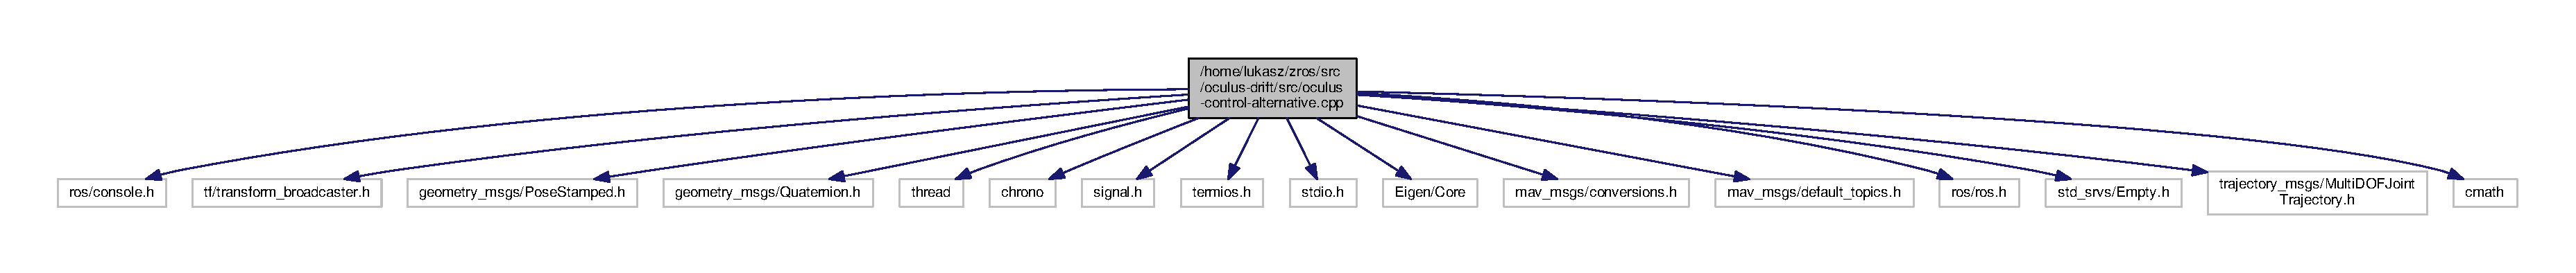
\includegraphics[width=350pt]{oculus-control-alternative_8cpp__incl}
\end{center}
\end{figure}
\subsection*{Functions}
\begin{DoxyCompactItemize}
\item 
Eigen\+::\+Vector3d \hyperlink{oculus-control-alternative_8cpp_a33ebb53f44ddfc738d5914aed4017e53}{desired\+\_\+position} (0.\+0, 0.\+0, 2.\+0)
\item 
void \hyperlink{oculus-control-alternative_8cpp_a570d60ef77ebe021853fd13c864ab969}{orientation\+Callback} (const geometry\+\_\+msgs\+::\+Quaternion\+::\+Const\+Ptr msg)
\item 
int \hyperlink{oculus-control-alternative_8cpp_a3c04138a5bfe5d72780bb7e82a18e627}{main} (int argc, char $\ast$$\ast$argv)
\end{DoxyCompactItemize}
\subsection*{Variables}
\begin{DoxyCompactItemize}
\item 
ros\+::\+Publisher \hyperlink{oculus-control-alternative_8cpp_a92b67ae724bc0d23b8e85e92e89403df}{pub\+\_\+traj}
\item 
trajectory\+\_\+msgs\+::\+Multi\+D\+O\+F\+Joint\+Trajectory \hyperlink{oculus-control-alternative_8cpp_a090c0766fbb77862dd8cc0cca99d688b}{traj\+\_\+msg}
\item 
geometry\+\_\+msgs\+::\+Quaternion \hyperlink{oculus-control-alternative_8cpp_a71181c8a89676b15be113f74f57c9f23}{quat}
\item 
float \hyperlink{oculus-control-alternative_8cpp_a7f7e4724cf57d59513b39c5ecc81adc8}{speed} = 0.\+1
\item 
double \hyperlink{oculus-control-alternative_8cpp_a03a69ef33d756512293e67791ab5f265}{desired\+\_\+yaw} = 0.\+0
\item 
double \hyperlink{oculus-control-alternative_8cpp_a6f2a069eeaa873686f0991fe351fec51}{old\+\_\+yaw} = 0.\+0
\begin{DoxyCompactList}\small\item\em The desired\+\_\+yaw. \end{DoxyCompactList}\item 
float \hyperlink{oculus-control-alternative_8cpp_a2cce9b626fdb3b1f78baad955bd5b609}{ninety\+Deg\+In\+Rad} = 1.\+5708
\end{DoxyCompactItemize}


\subsection{Function Documentation}
\index{oculus-\/control-\/alternative.\+cpp@{oculus-\/control-\/alternative.\+cpp}!desired\+\_\+position@{desired\+\_\+position}}
\index{desired\+\_\+position@{desired\+\_\+position}!oculus-\/control-\/alternative.\+cpp@{oculus-\/control-\/alternative.\+cpp}}
\subsubsection[{\texorpdfstring{desired\+\_\+position(0.\+0, 0.\+0, 2.\+0)}{desired_position(0.0, 0.0, 2.0)}}]{\setlength{\rightskip}{0pt plus 5cm}Eigen\+::\+Vector3d desired\+\_\+position (
\begin{DoxyParamCaption}
\item[{0.}]{0, }
\item[{0.}]{0, }
\item[{2.}]{0}
\end{DoxyParamCaption}
)}\hypertarget{oculus-control-alternative_8cpp_a33ebb53f44ddfc738d5914aed4017e53}{}\label{oculus-control-alternative_8cpp_a33ebb53f44ddfc738d5914aed4017e53}
\index{oculus-\/control-\/alternative.\+cpp@{oculus-\/control-\/alternative.\+cpp}!main@{main}}
\index{main@{main}!oculus-\/control-\/alternative.\+cpp@{oculus-\/control-\/alternative.\+cpp}}
\subsubsection[{\texorpdfstring{main(int argc, char $\ast$$\ast$argv)}{main(int argc, char **argv)}}]{\setlength{\rightskip}{0pt plus 5cm}int main (
\begin{DoxyParamCaption}
\item[{int}]{argc, }
\item[{char $\ast$$\ast$}]{argv}
\end{DoxyParamCaption}
)}\hypertarget{oculus-control-alternative_8cpp_a3c04138a5bfe5d72780bb7e82a18e627}{}\label{oculus-control-alternative_8cpp_a3c04138a5bfe5d72780bb7e82a18e627}

\begin{DoxyCode}
65 \{
66   ros::init(argc, argv, \textcolor{stringliteral}{"oculus\_control\_alternative"});
67   ros::NodeHandle nh;
68 
69   \hyperlink{oculus-control-alternative_8cpp_a090c0766fbb77862dd8cc0cca99d688b}{traj\_msg}.header.stamp = ros::Time::now();
70 
71   ros::Subscriber sub\_orient = nh.subscribe(\textcolor{stringliteral}{"/oculus/orientation"}, 1, 
      \hyperlink{oculus-control-alternative_8cpp_a570d60ef77ebe021853fd13c864ab969}{orientationCallback});
72 
73   \hyperlink{oculus-control-alternative_8cpp_a92b67ae724bc0d23b8e85e92e89403df}{pub\_traj} = nh.advertise<trajectory\_msgs::MultiDOFJointTrajectory>(\textcolor{stringliteral}{"/firefly/command/trajectory"}, 
      1);
74 
75   ros::Rate loop\_rate(5);
76   \textcolor{keywordflow}{while} (nh.ok()) \{
77 
78     ros::spinOnce();
79     loop\_rate.sleep();
80   \}
81 \}
\end{DoxyCode}
\index{oculus-\/control-\/alternative.\+cpp@{oculus-\/control-\/alternative.\+cpp}!orientation\+Callback@{orientation\+Callback}}
\index{orientation\+Callback@{orientation\+Callback}!oculus-\/control-\/alternative.\+cpp@{oculus-\/control-\/alternative.\+cpp}}
\subsubsection[{\texorpdfstring{orientation\+Callback(const geometry\+\_\+msgs\+::\+Quaternion\+::\+Const\+Ptr msg)}{orientationCallback(const geometry_msgs::Quaternion::ConstPtr msg)}}]{\setlength{\rightskip}{0pt plus 5cm}void orientation\+Callback (
\begin{DoxyParamCaption}
\item[{const geometry\+\_\+msgs\+::\+Quaternion\+::\+Const\+Ptr}]{msg}
\end{DoxyParamCaption}
)}\hypertarget{oculus-control-alternative_8cpp_a570d60ef77ebe021853fd13c864ab969}{}\label{oculus-control-alternative_8cpp_a570d60ef77ebe021853fd13c864ab969}

\begin{DoxyCode}
30 \{
31   ROS\_INFO(\textcolor{stringliteral}{"Callback Success"});
32 
33   \textcolor{keywordflow}{if} (msg->y < -0.2) \{
34     \hyperlink{oculus-control-alternative_8cpp_a03a69ef33d756512293e67791ab5f265}{desired\_yaw} = \hyperlink{oculus-control-alternative_8cpp_a03a69ef33d756512293e67791ab5f265}{desired\_yaw} - \hyperlink{oculus-control-alternative_8cpp_a7f7e4724cf57d59513b39c5ecc81adc8}{speed}/3;
35   \} \textcolor{keywordflow}{else} \textcolor{keywordflow}{if} (msg->y > 0.2) \{
36     \hyperlink{oculus-control-alternative_8cpp_a03a69ef33d756512293e67791ab5f265}{desired\_yaw} = \hyperlink{oculus-control-alternative_8cpp_a03a69ef33d756512293e67791ab5f265}{desired\_yaw} + \hyperlink{oculus-control-alternative_8cpp_a7f7e4724cf57d59513b39c5ecc81adc8}{speed}/3;
37   \}
38 
39   \textcolor{keywordflow}{if} (msg->x < -0.25) \{
40     \hyperlink{oculus-control-alternative_8cpp_a33ebb53f44ddfc738d5914aed4017e53}{desired\_position}.x() = \hyperlink{oculus-control-alternative_8cpp_a33ebb53f44ddfc738d5914aed4017e53}{desired\_position}.x() + 
      \hyperlink{oculus-control-alternative_8cpp_a7f7e4724cf57d59513b39c5ecc81adc8}{speed}*cos(\hyperlink{oculus-control-alternative_8cpp_a03a69ef33d756512293e67791ab5f265}{desired\_yaw});
41     \hyperlink{oculus-control-alternative_8cpp_a33ebb53f44ddfc738d5914aed4017e53}{desired\_position}.y() = \hyperlink{oculus-control-alternative_8cpp_a33ebb53f44ddfc738d5914aed4017e53}{desired\_position}.y() + 
      \hyperlink{oculus-control-alternative_8cpp_a7f7e4724cf57d59513b39c5ecc81adc8}{speed}*sin(\hyperlink{oculus-control-alternative_8cpp_a03a69ef33d756512293e67791ab5f265}{desired\_yaw});
42   \} \textcolor{keywordflow}{else} \textcolor{keywordflow}{if} (msg->x > 0.25) \{
43     \hyperlink{oculus-control-alternative_8cpp_a33ebb53f44ddfc738d5914aed4017e53}{desired\_position}.x() = \hyperlink{oculus-control-alternative_8cpp_a33ebb53f44ddfc738d5914aed4017e53}{desired\_position}.x() - 
      \hyperlink{oculus-control-alternative_8cpp_a7f7e4724cf57d59513b39c5ecc81adc8}{speed}*cos(\hyperlink{oculus-control-alternative_8cpp_a03a69ef33d756512293e67791ab5f265}{desired\_yaw});
44     \hyperlink{oculus-control-alternative_8cpp_a33ebb53f44ddfc738d5914aed4017e53}{desired\_position}.y() = \hyperlink{oculus-control-alternative_8cpp_a33ebb53f44ddfc738d5914aed4017e53}{desired\_position}.y() - 
      \hyperlink{oculus-control-alternative_8cpp_a7f7e4724cf57d59513b39c5ecc81adc8}{speed}*sin(\hyperlink{oculus-control-alternative_8cpp_a03a69ef33d756512293e67791ab5f265}{desired\_yaw});
45   \}
46 
47   \textcolor{keywordflow}{if} (msg->z < -0.25) \{
48     \hyperlink{oculus-control-alternative_8cpp_a33ebb53f44ddfc738d5914aed4017e53}{desired\_position}.x() = \hyperlink{oculus-control-alternative_8cpp_a33ebb53f44ddfc738d5914aed4017e53}{desired\_position}.x() + 
      \hyperlink{oculus-control-alternative_8cpp_a7f7e4724cf57d59513b39c5ecc81adc8}{speed}*cos(\hyperlink{oculus-control-alternative_8cpp_a03a69ef33d756512293e67791ab5f265}{desired\_yaw}-\hyperlink{oculus-control-alternative_8cpp_a2cce9b626fdb3b1f78baad955bd5b609}{ninetyDegInRad});
49     \hyperlink{oculus-control-alternative_8cpp_a33ebb53f44ddfc738d5914aed4017e53}{desired\_position}.y() = \hyperlink{oculus-control-alternative_8cpp_a33ebb53f44ddfc738d5914aed4017e53}{desired\_position}.y() + 
      \hyperlink{oculus-control-alternative_8cpp_a7f7e4724cf57d59513b39c5ecc81adc8}{speed}*sin(\hyperlink{oculus-control-alternative_8cpp_a03a69ef33d756512293e67791ab5f265}{desired\_yaw}-\hyperlink{oculus-control-alternative_8cpp_a2cce9b626fdb3b1f78baad955bd5b609}{ninetyDegInRad});
50   \} \textcolor{keywordflow}{else} \textcolor{keywordflow}{if} (msg->z > 0.25) \{
51     \hyperlink{oculus-control-alternative_8cpp_a33ebb53f44ddfc738d5914aed4017e53}{desired\_position}.x() = \hyperlink{oculus-control-alternative_8cpp_a33ebb53f44ddfc738d5914aed4017e53}{desired\_position}.x() - 
      \hyperlink{oculus-control-alternative_8cpp_a7f7e4724cf57d59513b39c5ecc81adc8}{speed}*cos(\hyperlink{oculus-control-alternative_8cpp_a03a69ef33d756512293e67791ab5f265}{desired\_yaw}-\hyperlink{oculus-control-alternative_8cpp_a2cce9b626fdb3b1f78baad955bd5b609}{ninetyDegInRad});
52     \hyperlink{oculus-control-alternative_8cpp_a33ebb53f44ddfc738d5914aed4017e53}{desired\_position}.y() = \hyperlink{oculus-control-alternative_8cpp_a33ebb53f44ddfc738d5914aed4017e53}{desired\_position}.y() - 
      \hyperlink{oculus-control-alternative_8cpp_a7f7e4724cf57d59513b39c5ecc81adc8}{speed}*sin(\hyperlink{oculus-control-alternative_8cpp_a03a69ef33d756512293e67791ab5f265}{desired\_yaw}-\hyperlink{oculus-control-alternative_8cpp_a2cce9b626fdb3b1f78baad955bd5b609}{ninetyDegInRad});
53   \}
54 
55   \hyperlink{oculus-control-alternative_8cpp_a6f2a069eeaa873686f0991fe351fec51}{old\_yaw} = \hyperlink{oculus-control-alternative_8cpp_a03a69ef33d756512293e67791ab5f265}{desired\_yaw};
56   mav\_msgs::msgMultiDofJointTrajectoryFromPositionYaw(\hyperlink{oculus-control-alternative_8cpp_a33ebb53f44ddfc738d5914aed4017e53}{desired\_position},
57       \hyperlink{oculus-control-alternative_8cpp_a03a69ef33d756512293e67791ab5f265}{desired\_yaw}, &\hyperlink{oculus-control-alternative_8cpp_a090c0766fbb77862dd8cc0cca99d688b}{traj\_msg});
58   \hyperlink{oculus-control-alternative_8cpp_a71181c8a89676b15be113f74f57c9f23}{quat} = *msg;
59   \hyperlink{oculus-control-alternative_8cpp_a92b67ae724bc0d23b8e85e92e89403df}{pub\_traj}.publish(\hyperlink{oculus-control-alternative_8cpp_a090c0766fbb77862dd8cc0cca99d688b}{traj\_msg});
60 
61 \}
\end{DoxyCode}


\subsection{Variable Documentation}
\index{oculus-\/control-\/alternative.\+cpp@{oculus-\/control-\/alternative.\+cpp}!desired\+\_\+yaw@{desired\+\_\+yaw}}
\index{desired\+\_\+yaw@{desired\+\_\+yaw}!oculus-\/control-\/alternative.\+cpp@{oculus-\/control-\/alternative.\+cpp}}
\subsubsection[{\texorpdfstring{desired\+\_\+yaw}{desired_yaw}}]{\setlength{\rightskip}{0pt plus 5cm}double desired\+\_\+yaw = 0.\+0}\hypertarget{oculus-control-alternative_8cpp_a03a69ef33d756512293e67791ab5f265}{}\label{oculus-control-alternative_8cpp_a03a69ef33d756512293e67791ab5f265}
\index{oculus-\/control-\/alternative.\+cpp@{oculus-\/control-\/alternative.\+cpp}!ninety\+Deg\+In\+Rad@{ninety\+Deg\+In\+Rad}}
\index{ninety\+Deg\+In\+Rad@{ninety\+Deg\+In\+Rad}!oculus-\/control-\/alternative.\+cpp@{oculus-\/control-\/alternative.\+cpp}}
\subsubsection[{\texorpdfstring{ninety\+Deg\+In\+Rad}{ninetyDegInRad}}]{\setlength{\rightskip}{0pt plus 5cm}float ninety\+Deg\+In\+Rad = 1.\+5708}\hypertarget{oculus-control-alternative_8cpp_a2cce9b626fdb3b1f78baad955bd5b609}{}\label{oculus-control-alternative_8cpp_a2cce9b626fdb3b1f78baad955bd5b609}
\index{oculus-\/control-\/alternative.\+cpp@{oculus-\/control-\/alternative.\+cpp}!old\+\_\+yaw@{old\+\_\+yaw}}
\index{old\+\_\+yaw@{old\+\_\+yaw}!oculus-\/control-\/alternative.\+cpp@{oculus-\/control-\/alternative.\+cpp}}
\subsubsection[{\texorpdfstring{old\+\_\+yaw}{old_yaw}}]{\setlength{\rightskip}{0pt plus 5cm}double old\+\_\+yaw = 0.\+0}\hypertarget{oculus-control-alternative_8cpp_a6f2a069eeaa873686f0991fe351fec51}{}\label{oculus-control-alternative_8cpp_a6f2a069eeaa873686f0991fe351fec51}


The desired\+\_\+yaw. 

\index{oculus-\/control-\/alternative.\+cpp@{oculus-\/control-\/alternative.\+cpp}!pub\+\_\+traj@{pub\+\_\+traj}}
\index{pub\+\_\+traj@{pub\+\_\+traj}!oculus-\/control-\/alternative.\+cpp@{oculus-\/control-\/alternative.\+cpp}}
\subsubsection[{\texorpdfstring{pub\+\_\+traj}{pub_traj}}]{\setlength{\rightskip}{0pt plus 5cm}ros\+::\+Publisher pub\+\_\+traj}\hypertarget{oculus-control-alternative_8cpp_a92b67ae724bc0d23b8e85e92e89403df}{}\label{oculus-control-alternative_8cpp_a92b67ae724bc0d23b8e85e92e89403df}
\index{oculus-\/control-\/alternative.\+cpp@{oculus-\/control-\/alternative.\+cpp}!quat@{quat}}
\index{quat@{quat}!oculus-\/control-\/alternative.\+cpp@{oculus-\/control-\/alternative.\+cpp}}
\subsubsection[{\texorpdfstring{quat}{quat}}]{\setlength{\rightskip}{0pt plus 5cm}geometry\+\_\+msgs\+::\+Quaternion quat}\hypertarget{oculus-control-alternative_8cpp_a71181c8a89676b15be113f74f57c9f23}{}\label{oculus-control-alternative_8cpp_a71181c8a89676b15be113f74f57c9f23}
\index{oculus-\/control-\/alternative.\+cpp@{oculus-\/control-\/alternative.\+cpp}!speed@{speed}}
\index{speed@{speed}!oculus-\/control-\/alternative.\+cpp@{oculus-\/control-\/alternative.\+cpp}}
\subsubsection[{\texorpdfstring{speed}{speed}}]{\setlength{\rightskip}{0pt plus 5cm}float speed = 0.\+1}\hypertarget{oculus-control-alternative_8cpp_a7f7e4724cf57d59513b39c5ecc81adc8}{}\label{oculus-control-alternative_8cpp_a7f7e4724cf57d59513b39c5ecc81adc8}
\index{oculus-\/control-\/alternative.\+cpp@{oculus-\/control-\/alternative.\+cpp}!traj\+\_\+msg@{traj\+\_\+msg}}
\index{traj\+\_\+msg@{traj\+\_\+msg}!oculus-\/control-\/alternative.\+cpp@{oculus-\/control-\/alternative.\+cpp}}
\subsubsection[{\texorpdfstring{traj\+\_\+msg}{traj_msg}}]{\setlength{\rightskip}{0pt plus 5cm}trajectory\+\_\+msgs\+::\+Multi\+D\+O\+F\+Joint\+Trajectory traj\+\_\+msg}\hypertarget{oculus-control-alternative_8cpp_a090c0766fbb77862dd8cc0cca99d688b}{}\label{oculus-control-alternative_8cpp_a090c0766fbb77862dd8cc0cca99d688b}

\hypertarget{oculus-control-keyboard_8cpp}{}\section{/home/lukasz/zros/src/oculus-\/drift/src/oculus-\/control-\/keyboard.cpp File Reference}
\label{oculus-control-keyboard_8cpp}\index{/home/lukasz/zros/src/oculus-\/drift/src/oculus-\/control-\/keyboard.\+cpp@{/home/lukasz/zros/src/oculus-\/drift/src/oculus-\/control-\/keyboard.\+cpp}}
{\ttfamily \#include $<$ros/console.\+h$>$}\\*
{\ttfamily \#include $<$tf/transform\+\_\+broadcaster.\+h$>$}\\*
{\ttfamily \#include \char`\"{}geometry\+\_\+msgs/\+Pose\+Stamped.\+h\char`\"{}}\\*
{\ttfamily \#include \char`\"{}geometry\+\_\+msgs/\+Quaternion.\+h\char`\"{}}\\*
{\ttfamily \#include $<$thread$>$}\\*
{\ttfamily \#include $<$chrono$>$}\\*
{\ttfamily \#include $<$signal.\+h$>$}\\*
{\ttfamily \#include $<$termios.\+h$>$}\\*
{\ttfamily \#include $<$stdio.\+h$>$}\\*
{\ttfamily \#include $<$Eigen/\+Core$>$}\\*
{\ttfamily \#include $<$mav\+\_\+msgs/conversions.\+h$>$}\\*
{\ttfamily \#include $<$mav\+\_\+msgs/default\+\_\+topics.\+h$>$}\\*
{\ttfamily \#include $<$ros/ros.\+h$>$}\\*
{\ttfamily \#include $<$std\+\_\+srvs/\+Empty.\+h$>$}\\*
{\ttfamily \#include $<$trajectory\+\_\+msgs/\+Multi\+D\+O\+F\+Joint\+Trajectory.\+h$>$}\\*
{\ttfamily \#include $<$cmath$>$}\\*
Include dependency graph for oculus-\/control-\/keyboard.cpp\+:\nopagebreak
\begin{figure}[H]
\begin{center}
\leavevmode
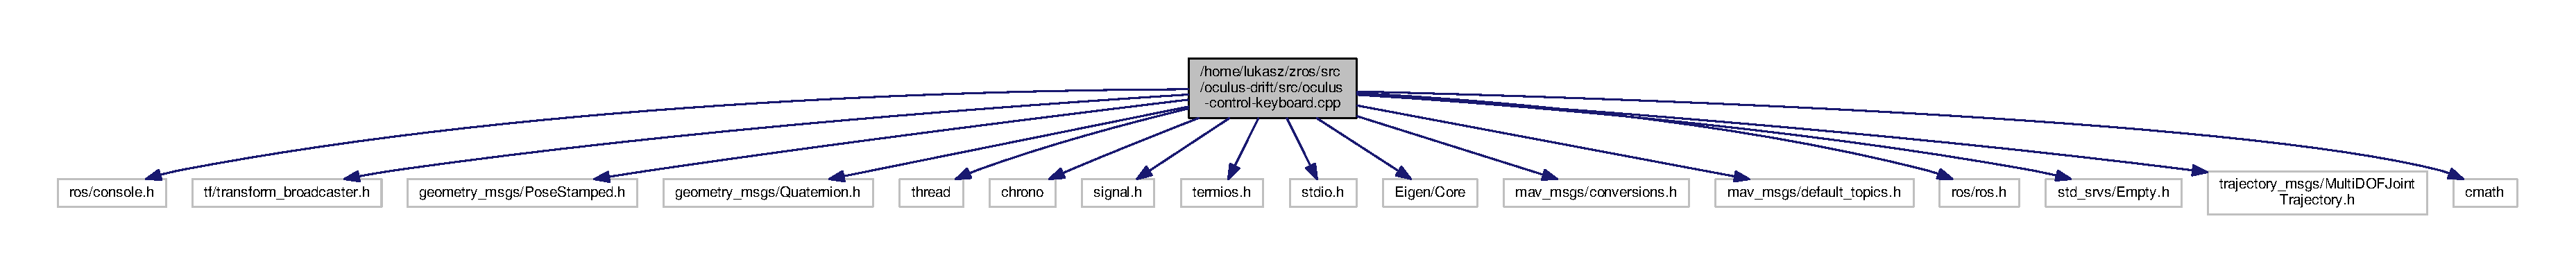
\includegraphics[width=350pt]{oculus-control-keyboard_8cpp__incl}
\end{center}
\end{figure}
\subsection*{Functions}
\begin{DoxyCompactItemize}
\item 
Eigen\+::\+Vector3d \hyperlink{oculus-control-keyboard_8cpp_a608d9948c063034b7605598daaeccc3e}{desired\+\_\+position} (0.\+0, 0.\+0, 1.\+0)
\item 
int \hyperlink{oculus-control-keyboard_8cpp_a3c04138a5bfe5d72780bb7e82a18e627}{main} (int argc, char $\ast$$\ast$argv)
\end{DoxyCompactItemize}
\subsection*{Variables}
\begin{DoxyCompactItemize}
\item 
ros\+::\+Publisher \hyperlink{oculus-control-keyboard_8cpp_a92b67ae724bc0d23b8e85e92e89403df}{pub\+\_\+traj}
\item 
trajectory\+\_\+msgs\+::\+Multi\+D\+O\+F\+Joint\+Trajectory \hyperlink{oculus-control-keyboard_8cpp_a090c0766fbb77862dd8cc0cca99d688b}{traj\+\_\+msg}
\item 
float \hyperlink{oculus-control-keyboard_8cpp_a7f7e4724cf57d59513b39c5ecc81adc8}{speed} = 0.\+1
\item 
float \hyperlink{oculus-control-keyboard_8cpp_a2cce9b626fdb3b1f78baad955bd5b609}{ninety\+Deg\+In\+Rad} = 1.\+5708
\item 
double \hyperlink{oculus-control-keyboard_8cpp_a03a69ef33d756512293e67791ab5f265}{desired\+\_\+yaw} = 0.\+0
\end{DoxyCompactItemize}


\subsection{Function Documentation}
\index{oculus-\/control-\/keyboard.\+cpp@{oculus-\/control-\/keyboard.\+cpp}!desired\+\_\+position@{desired\+\_\+position}}
\index{desired\+\_\+position@{desired\+\_\+position}!oculus-\/control-\/keyboard.\+cpp@{oculus-\/control-\/keyboard.\+cpp}}
\subsubsection[{\texorpdfstring{desired\+\_\+position(0.\+0, 0.\+0, 1.\+0)}{desired_position(0.0, 0.0, 1.0)}}]{\setlength{\rightskip}{0pt plus 5cm}Eigen\+::\+Vector3d desired\+\_\+position (
\begin{DoxyParamCaption}
\item[{0.}]{0, }
\item[{0.}]{0, }
\item[{1.}]{0}
\end{DoxyParamCaption}
)}\hypertarget{oculus-control-keyboard_8cpp_a608d9948c063034b7605598daaeccc3e}{}\label{oculus-control-keyboard_8cpp_a608d9948c063034b7605598daaeccc3e}
\index{oculus-\/control-\/keyboard.\+cpp@{oculus-\/control-\/keyboard.\+cpp}!main@{main}}
\index{main@{main}!oculus-\/control-\/keyboard.\+cpp@{oculus-\/control-\/keyboard.\+cpp}}
\subsubsection[{\texorpdfstring{main(int argc, char $\ast$$\ast$argv)}{main(int argc, char **argv)}}]{\setlength{\rightskip}{0pt plus 5cm}int main (
\begin{DoxyParamCaption}
\item[{int}]{argc, }
\item[{char $\ast$$\ast$}]{argv}
\end{DoxyParamCaption}
)}\hypertarget{oculus-control-keyboard_8cpp_a3c04138a5bfe5d72780bb7e82a18e627}{}\label{oculus-control-keyboard_8cpp_a3c04138a5bfe5d72780bb7e82a18e627}

\begin{DoxyCode}
28 \{
29   ros::init(argc, argv, \textcolor{stringliteral}{"oculus\_keycontrol"});
30   ros::NodeHandle nh;
31   \hyperlink{oculus-control-keyboard_8cpp_a090c0766fbb77862dd8cc0cca99d688b}{traj\_msg}.header.stamp = ros::Time::now();
32 
33   \hyperlink{oculus-control-keyboard_8cpp_a92b67ae724bc0d23b8e85e92e89403df}{pub\_traj} = nh.advertise<trajectory\_msgs::MultiDOFJointTrajectory>(\textcolor{stringliteral}{"/firefly/command/trajectory"}, 
      1);
34 
35   \textcolor{keywordtype}{int} ch, oldch;
36   \textcolor{keywordtype}{char} cheese;
37   \textcolor{keywordtype}{int} kfd = 0;
38   \textcolor{keyword}{struct }termios cooked, raw;
39   \textcolor{keywordtype}{float} \hyperlink{oculus-control-keyboard_8cpp_a7f7e4724cf57d59513b39c5ecc81adc8}{speed} = 0.05;
40   \textcolor{keywordtype}{int} active = 0;
41 
42 
43   \textcolor{keywordflow}{while}(1) \{
44 
45     \textcolor{comment}{// get the console in raw mode}
46     tcgetattr(kfd, &cooked);
47     memcpy(&raw, &cooked, \textcolor{keyword}{sizeof}(\textcolor{keyword}{struct} termios));
48     raw.c\_lflag &=~ (ICANON | ECHO);
49     \textcolor{comment}{// Setting a new line, then end of file}
50     raw.c\_cc[VEOL] = 1;
51     raw.c\_cc[VEOF] = 2;
52     tcsetattr(kfd, TCSANOW, &raw);
53 
54     puts(\textcolor{stringliteral}{"Reading from keyboard"});
55     puts(\textcolor{stringliteral}{"----Press X to activate/deactivate control-----------------"});
56     puts(\textcolor{stringliteral}{"Use W,A,S,D to move the drone. Use Q,E to adjust height of the drone. R,F to rotate."});
57 
58     \textcolor{keywordflow}{if}(read(kfd, &cheese, 1) < 0)
59     \{
60       perror(\textcolor{stringliteral}{"read():"});
61       exit(-1);
62     \}
63 
64 
65     \textcolor{keywordflow}{switch} (cheese) \{
66       \textcolor{keywordflow}{case} \textcolor{charliteral}{'x'}:
67       \textcolor{keywordflow}{case} \textcolor{charliteral}{'X'}:
68         \textcolor{keywordflow}{if}(active == 0) \{
69           active = 1;
70         \} \textcolor{keywordflow}{else} \{
71           active = 0;
72         \}
73       \textcolor{keywordflow}{case} \textcolor{charliteral}{'a'}:
74       \textcolor{keywordflow}{case} \textcolor{charliteral}{'A'}:
75         ROS\_INFO(\textcolor{stringliteral}{"A"});
76         \hyperlink{oculus-control-keyboard_8cpp_a608d9948c063034b7605598daaeccc3e}{desired\_position}.x() = \hyperlink{oculus-control-keyboard_8cpp_a608d9948c063034b7605598daaeccc3e}{desired\_position}.x() - speed*cos(
      \hyperlink{oculus-control-keyboard_8cpp_a03a69ef33d756512293e67791ab5f265}{desired\_yaw}-\hyperlink{oculus-control-keyboard_8cpp_a2cce9b626fdb3b1f78baad955bd5b609}{ninetyDegInRad});
77         \hyperlink{oculus-control-keyboard_8cpp_a608d9948c063034b7605598daaeccc3e}{desired\_position}.y() = \hyperlink{oculus-control-keyboard_8cpp_a608d9948c063034b7605598daaeccc3e}{desired\_position}.y() - speed*sin(
      \hyperlink{oculus-control-keyboard_8cpp_a03a69ef33d756512293e67791ab5f265}{desired\_yaw}-\hyperlink{oculus-control-keyboard_8cpp_a2cce9b626fdb3b1f78baad955bd5b609}{ninetyDegInRad});
78         \textcolor{keywordflow}{goto} PUB;
79         \textcolor{keywordflow}{break};
80       \textcolor{keywordflow}{case} \textcolor{charliteral}{'s'}:
81       \textcolor{keywordflow}{case} \textcolor{charliteral}{'S'}:
82         ROS\_INFO(\textcolor{stringliteral}{"S"});
83         \hyperlink{oculus-control-keyboard_8cpp_a608d9948c063034b7605598daaeccc3e}{desired\_position}.x() = \hyperlink{oculus-control-keyboard_8cpp_a608d9948c063034b7605598daaeccc3e}{desired\_position}.x() - speed*cos(
      \hyperlink{oculus-control-keyboard_8cpp_a03a69ef33d756512293e67791ab5f265}{desired\_yaw});
84         \hyperlink{oculus-control-keyboard_8cpp_a608d9948c063034b7605598daaeccc3e}{desired\_position}.y() = \hyperlink{oculus-control-keyboard_8cpp_a608d9948c063034b7605598daaeccc3e}{desired\_position}.y() - speed*sin(
      \hyperlink{oculus-control-keyboard_8cpp_a03a69ef33d756512293e67791ab5f265}{desired\_yaw});
85         \textcolor{keywordflow}{goto} PUB;
86         \textcolor{keywordflow}{break};
87       \textcolor{keywordflow}{case} \textcolor{charliteral}{'d'}:
88       \textcolor{keywordflow}{case} \textcolor{charliteral}{'D'}:
89         ROS\_INFO(\textcolor{stringliteral}{"D"});
90         \hyperlink{oculus-control-keyboard_8cpp_a608d9948c063034b7605598daaeccc3e}{desired\_position}.x() = \hyperlink{oculus-control-keyboard_8cpp_a608d9948c063034b7605598daaeccc3e}{desired\_position}.x() + speed*cos(
      \hyperlink{oculus-control-keyboard_8cpp_a03a69ef33d756512293e67791ab5f265}{desired\_yaw}-\hyperlink{oculus-control-keyboard_8cpp_a2cce9b626fdb3b1f78baad955bd5b609}{ninetyDegInRad});
91         \hyperlink{oculus-control-keyboard_8cpp_a608d9948c063034b7605598daaeccc3e}{desired\_position}.y() = \hyperlink{oculus-control-keyboard_8cpp_a608d9948c063034b7605598daaeccc3e}{desired\_position}.y() + speed*sin(
      \hyperlink{oculus-control-keyboard_8cpp_a03a69ef33d756512293e67791ab5f265}{desired\_yaw}-\hyperlink{oculus-control-keyboard_8cpp_a2cce9b626fdb3b1f78baad955bd5b609}{ninetyDegInRad});
92         \textcolor{keywordflow}{goto} PUB;
93         \textcolor{keywordflow}{break};
94       \textcolor{keywordflow}{case} \textcolor{charliteral}{'w'}:
95       \textcolor{keywordflow}{case} \textcolor{charliteral}{'W'}:
96         ROS\_INFO(\textcolor{stringliteral}{"W"});
97         \hyperlink{oculus-control-keyboard_8cpp_a608d9948c063034b7605598daaeccc3e}{desired\_position}.x() = \hyperlink{oculus-control-keyboard_8cpp_a608d9948c063034b7605598daaeccc3e}{desired\_position}.x() + speed*cos(
      \hyperlink{oculus-control-keyboard_8cpp_a03a69ef33d756512293e67791ab5f265}{desired\_yaw});
98         \hyperlink{oculus-control-keyboard_8cpp_a608d9948c063034b7605598daaeccc3e}{desired\_position}.y() = \hyperlink{oculus-control-keyboard_8cpp_a608d9948c063034b7605598daaeccc3e}{desired\_position}.y() + speed*sin(
      \hyperlink{oculus-control-keyboard_8cpp_a03a69ef33d756512293e67791ab5f265}{desired\_yaw});
99         \textcolor{keywordflow}{goto} PUB;
100         \textcolor{keywordflow}{break};
101       \textcolor{keywordflow}{case} \textcolor{charliteral}{'q'}:
102       \textcolor{keywordflow}{case} \textcolor{charliteral}{'Q'}:
103         ROS\_INFO(\textcolor{stringliteral}{"Q"});
104         \hyperlink{oculus-control-keyboard_8cpp_a608d9948c063034b7605598daaeccc3e}{desired\_position}.z() = \hyperlink{oculus-control-keyboard_8cpp_a608d9948c063034b7605598daaeccc3e}{desired\_position}.z() + 
      \hyperlink{oculus-control-keyboard_8cpp_a7f7e4724cf57d59513b39c5ecc81adc8}{speed};
105         \textcolor{keywordflow}{goto} PUB;
106         \textcolor{keywordflow}{break};
107       \textcolor{keywordflow}{case} \textcolor{charliteral}{'e'}:
108       \textcolor{keywordflow}{case} \textcolor{charliteral}{'E'}:
109         ROS\_INFO(\textcolor{stringliteral}{"E"});
110         \hyperlink{oculus-control-keyboard_8cpp_a608d9948c063034b7605598daaeccc3e}{desired\_position}.z() = \hyperlink{oculus-control-keyboard_8cpp_a608d9948c063034b7605598daaeccc3e}{desired\_position}.z() - 
      \hyperlink{oculus-control-keyboard_8cpp_a7f7e4724cf57d59513b39c5ecc81adc8}{speed};
111         \textcolor{keywordflow}{goto} PUB;
112         \textcolor{keywordflow}{break};
113       \textcolor{keywordflow}{case} \textcolor{charliteral}{'r'}:
114       \textcolor{keywordflow}{case} \textcolor{charliteral}{'R'}:
115         ROS\_INFO(\textcolor{stringliteral}{"R"});
116         \hyperlink{oculus-control-keyboard_8cpp_a03a69ef33d756512293e67791ab5f265}{desired\_yaw} = \hyperlink{oculus-control-keyboard_8cpp_a03a69ef33d756512293e67791ab5f265}{desired\_yaw} + \hyperlink{oculus-control-keyboard_8cpp_a7f7e4724cf57d59513b39c5ecc81adc8}{speed};
117         \textcolor{keywordflow}{goto} PUB;
118         \textcolor{keywordflow}{break};
119       \textcolor{keywordflow}{case} \textcolor{charliteral}{'f'}:
120       \textcolor{keywordflow}{case} \textcolor{charliteral}{'F'}:
121         ROS\_INFO(\textcolor{stringliteral}{"F"});
122         \hyperlink{oculus-control-keyboard_8cpp_a03a69ef33d756512293e67791ab5f265}{desired\_yaw} = \hyperlink{oculus-control-keyboard_8cpp_a03a69ef33d756512293e67791ab5f265}{desired\_yaw} - \hyperlink{oculus-control-keyboard_8cpp_a7f7e4724cf57d59513b39c5ecc81adc8}{speed};
123         \textcolor{keywordflow}{goto} PUB;
124         \textcolor{keywordflow}{break};
125 
126       PUB:
127         \textcolor{keywordflow}{if} (active) \{
128           ROS\_INFO(\textcolor{stringliteral}{"publishing"});
129               mav\_msgs::msgMultiDofJointTrajectoryFromPositionYaw(
      \hyperlink{oculus-control-keyboard_8cpp_a608d9948c063034b7605598daaeccc3e}{desired\_position},
130                   \hyperlink{oculus-control-keyboard_8cpp_a03a69ef33d756512293e67791ab5f265}{desired\_yaw}, &\hyperlink{oculus-control-keyboard_8cpp_a090c0766fbb77862dd8cc0cca99d688b}{traj\_msg});
131           \hyperlink{oculus-control-keyboard_8cpp_a92b67ae724bc0d23b8e85e92e89403df}{pub\_traj}.publish(\hyperlink{oculus-control-keyboard_8cpp_a090c0766fbb77862dd8cc0cca99d688b}{traj\_msg});
132         \}
133       \}
134     \}
135 \}
\end{DoxyCode}


\subsection{Variable Documentation}
\index{oculus-\/control-\/keyboard.\+cpp@{oculus-\/control-\/keyboard.\+cpp}!desired\+\_\+yaw@{desired\+\_\+yaw}}
\index{desired\+\_\+yaw@{desired\+\_\+yaw}!oculus-\/control-\/keyboard.\+cpp@{oculus-\/control-\/keyboard.\+cpp}}
\subsubsection[{\texorpdfstring{desired\+\_\+yaw}{desired_yaw}}]{\setlength{\rightskip}{0pt plus 5cm}double desired\+\_\+yaw = 0.\+0}\hypertarget{oculus-control-keyboard_8cpp_a03a69ef33d756512293e67791ab5f265}{}\label{oculus-control-keyboard_8cpp_a03a69ef33d756512293e67791ab5f265}
\index{oculus-\/control-\/keyboard.\+cpp@{oculus-\/control-\/keyboard.\+cpp}!ninety\+Deg\+In\+Rad@{ninety\+Deg\+In\+Rad}}
\index{ninety\+Deg\+In\+Rad@{ninety\+Deg\+In\+Rad}!oculus-\/control-\/keyboard.\+cpp@{oculus-\/control-\/keyboard.\+cpp}}
\subsubsection[{\texorpdfstring{ninety\+Deg\+In\+Rad}{ninetyDegInRad}}]{\setlength{\rightskip}{0pt plus 5cm}float ninety\+Deg\+In\+Rad = 1.\+5708}\hypertarget{oculus-control-keyboard_8cpp_a2cce9b626fdb3b1f78baad955bd5b609}{}\label{oculus-control-keyboard_8cpp_a2cce9b626fdb3b1f78baad955bd5b609}
\index{oculus-\/control-\/keyboard.\+cpp@{oculus-\/control-\/keyboard.\+cpp}!pub\+\_\+traj@{pub\+\_\+traj}}
\index{pub\+\_\+traj@{pub\+\_\+traj}!oculus-\/control-\/keyboard.\+cpp@{oculus-\/control-\/keyboard.\+cpp}}
\subsubsection[{\texorpdfstring{pub\+\_\+traj}{pub_traj}}]{\setlength{\rightskip}{0pt plus 5cm}ros\+::\+Publisher pub\+\_\+traj}\hypertarget{oculus-control-keyboard_8cpp_a92b67ae724bc0d23b8e85e92e89403df}{}\label{oculus-control-keyboard_8cpp_a92b67ae724bc0d23b8e85e92e89403df}
\index{oculus-\/control-\/keyboard.\+cpp@{oculus-\/control-\/keyboard.\+cpp}!speed@{speed}}
\index{speed@{speed}!oculus-\/control-\/keyboard.\+cpp@{oculus-\/control-\/keyboard.\+cpp}}
\subsubsection[{\texorpdfstring{speed}{speed}}]{\setlength{\rightskip}{0pt plus 5cm}float speed = 0.\+1}\hypertarget{oculus-control-keyboard_8cpp_a7f7e4724cf57d59513b39c5ecc81adc8}{}\label{oculus-control-keyboard_8cpp_a7f7e4724cf57d59513b39c5ecc81adc8}
\index{oculus-\/control-\/keyboard.\+cpp@{oculus-\/control-\/keyboard.\+cpp}!traj\+\_\+msg@{traj\+\_\+msg}}
\index{traj\+\_\+msg@{traj\+\_\+msg}!oculus-\/control-\/keyboard.\+cpp@{oculus-\/control-\/keyboard.\+cpp}}
\subsubsection[{\texorpdfstring{traj\+\_\+msg}{traj_msg}}]{\setlength{\rightskip}{0pt plus 5cm}trajectory\+\_\+msgs\+::\+Multi\+D\+O\+F\+Joint\+Trajectory traj\+\_\+msg}\hypertarget{oculus-control-keyboard_8cpp_a090c0766fbb77862dd8cc0cca99d688b}{}\label{oculus-control-keyboard_8cpp_a090c0766fbb77862dd8cc0cca99d688b}

\hypertarget{oculus-control_8cpp}{}\section{/home/lukasz/zros/src/oculus-\/drift/src/oculus-\/control.cpp File Reference}
\label{oculus-control_8cpp}\index{/home/lukasz/zros/src/oculus-\/drift/src/oculus-\/control.\+cpp@{/home/lukasz/zros/src/oculus-\/drift/src/oculus-\/control.\+cpp}}
{\ttfamily \#include $<$ros/console.\+h$>$}\\*
{\ttfamily \#include $<$tf/transform\+\_\+broadcaster.\+h$>$}\\*
{\ttfamily \#include \char`\"{}geometry\+\_\+msgs/\+Pose\+Stamped.\+h\char`\"{}}\\*
{\ttfamily \#include \char`\"{}geometry\+\_\+msgs/\+Quaternion.\+h\char`\"{}}\\*
{\ttfamily \#include $<$thread$>$}\\*
{\ttfamily \#include $<$chrono$>$}\\*
{\ttfamily \#include $<$signal.\+h$>$}\\*
{\ttfamily \#include $<$termios.\+h$>$}\\*
{\ttfamily \#include $<$stdio.\+h$>$}\\*
{\ttfamily \#include $<$Eigen/\+Core$>$}\\*
{\ttfamily \#include $<$mav\+\_\+msgs/conversions.\+h$>$}\\*
{\ttfamily \#include $<$mav\+\_\+msgs/default\+\_\+topics.\+h$>$}\\*
{\ttfamily \#include $<$ros/ros.\+h$>$}\\*
{\ttfamily \#include $<$std\+\_\+srvs/\+Empty.\+h$>$}\\*
{\ttfamily \#include $<$trajectory\+\_\+msgs/\+Multi\+D\+O\+F\+Joint\+Trajectory.\+h$>$}\\*
{\ttfamily \#include $<$cmath$>$}\\*
Include dependency graph for oculus-\/control.cpp\+:\nopagebreak
\begin{figure}[H]
\begin{center}
\leavevmode
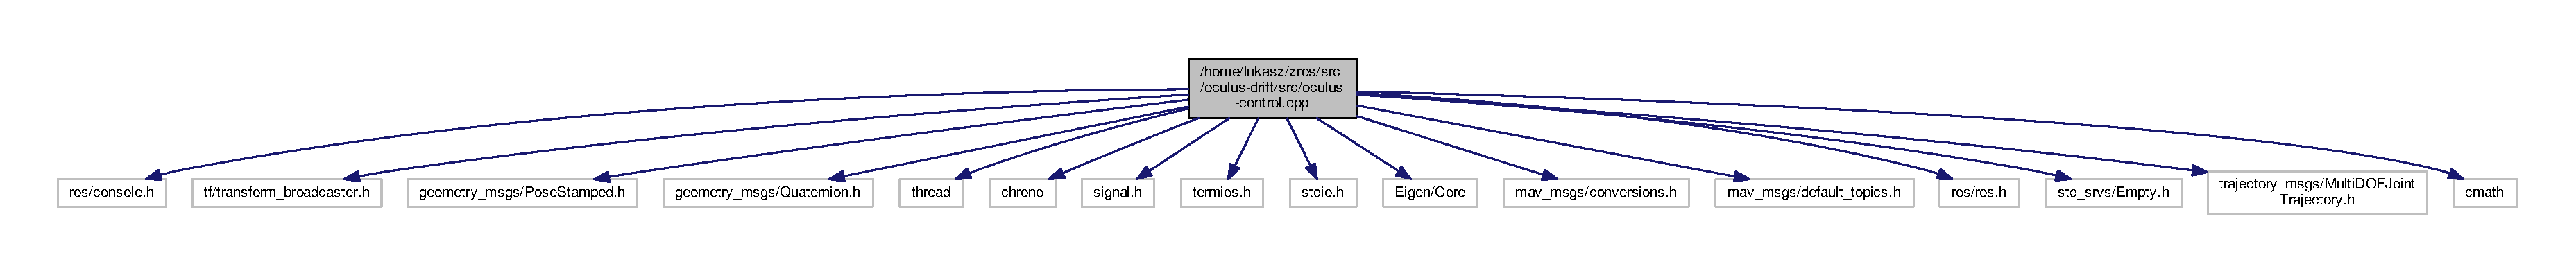
\includegraphics[width=350pt]{oculus-control_8cpp__incl}
\end{center}
\end{figure}
\subsection*{Functions}
\begin{DoxyCompactItemize}
\item 
Eigen\+::\+Vector3d \hyperlink{oculus-control_8cpp_a608d9948c063034b7605598daaeccc3e}{desired\+\_\+position} (0.\+0, 0.\+0, 1.\+0)
\begin{DoxyCompactList}\small\item\em The position the drone is expected to go to. \end{DoxyCompactList}\item 
void \hyperlink{oculus-control_8cpp_a570d60ef77ebe021853fd13c864ab969}{orientation\+Callback} (const geometry\+\_\+msgs\+::\+Quaternion\+::\+Const\+Ptr msg)
\begin{DoxyCompactList}\small\item\em Callback Function for Oculus Orientation Information. \end{DoxyCompactList}\item 
int \hyperlink{oculus-control_8cpp_a3c04138a5bfe5d72780bb7e82a18e627}{main} (int argc, char $\ast$$\ast$argv)
\begin{DoxyCompactList}\small\item\em Main function. \end{DoxyCompactList}\end{DoxyCompactItemize}
\subsection*{Variables}
\begin{DoxyCompactItemize}
\item 
ros\+::\+Publisher \hyperlink{oculus-control_8cpp_a92b67ae724bc0d23b8e85e92e89403df}{pub\+\_\+traj}
\begin{DoxyCompactList}\small\item\em Publisher for the desired trajectory of the drone. \end{DoxyCompactList}\item 
trajectory\+\_\+msgs\+::\+Multi\+D\+O\+F\+Joint\+Trajectory \hyperlink{oculus-control_8cpp_a090c0766fbb77862dd8cc0cca99d688b}{traj\+\_\+msg}
\begin{DoxyCompactList}\small\item\em The message variable that is published. \end{DoxyCompactList}\item 
float \hyperlink{oculus-control_8cpp_a7f7e4724cf57d59513b39c5ecc81adc8}{speed} = 0.\+1
\begin{DoxyCompactList}\small\item\em The speed at which the drone can move at. \end{DoxyCompactList}\item 
float \hyperlink{oculus-control_8cpp_a2cce9b626fdb3b1f78baad955bd5b609}{ninety\+Deg\+In\+Rad} = 1.\+5708
\begin{DoxyCompactList}\small\item\em The value 90 degrees holds in radians (rounded) \end{DoxyCompactList}\item 
double \hyperlink{oculus-control_8cpp_a03a69ef33d756512293e67791ab5f265}{desired\+\_\+yaw} = 0.\+0
\begin{DoxyCompactList}\small\item\em The yaw rotation expected of the drone to turn to (in radians) \end{DoxyCompactList}\end{DoxyCompactItemize}


\subsection{Function Documentation}
\index{oculus-\/control.\+cpp@{oculus-\/control.\+cpp}!desired\+\_\+position@{desired\+\_\+position}}
\index{desired\+\_\+position@{desired\+\_\+position}!oculus-\/control.\+cpp@{oculus-\/control.\+cpp}}
\subsubsection[{\texorpdfstring{desired\+\_\+position(0.\+0, 0.\+0, 1.\+0)}{desired_position(0.0, 0.0, 1.0)}}]{\setlength{\rightskip}{0pt plus 5cm}Eigen\+::\+Vector3d desired\+\_\+position (
\begin{DoxyParamCaption}
\item[{0.}]{0, }
\item[{0.}]{0, }
\item[{1.}]{0}
\end{DoxyParamCaption}
)}\hypertarget{oculus-control_8cpp_a608d9948c063034b7605598daaeccc3e}{}\label{oculus-control_8cpp_a608d9948c063034b7605598daaeccc3e}


The position the drone is expected to go to. 

\index{oculus-\/control.\+cpp@{oculus-\/control.\+cpp}!main@{main}}
\index{main@{main}!oculus-\/control.\+cpp@{oculus-\/control.\+cpp}}
\subsubsection[{\texorpdfstring{main(int argc, char $\ast$$\ast$argv)}{main(int argc, char **argv)}}]{\setlength{\rightskip}{0pt plus 5cm}int main (
\begin{DoxyParamCaption}
\item[{int}]{argc, }
\item[{char $\ast$$\ast$}]{argv}
\end{DoxyParamCaption}
)}\hypertarget{oculus-control_8cpp_a3c04138a5bfe5d72780bb7e82a18e627}{}\label{oculus-control_8cpp_a3c04138a5bfe5d72780bb7e82a18e627}


Main function. 

That setups up the subscription to the oculus\textquotesingle{}s orientation and the publisher to the firefly drone. 
\begin{DoxyCode}
89 \{
90   ros::init(argc, argv, \textcolor{stringliteral}{"oculus\_control"});
91   ros::NodeHandle nh;
92 
93   \hyperlink{oculus-control_8cpp_a090c0766fbb77862dd8cc0cca99d688b}{traj\_msg}.header.stamp = ros::Time::now();
94 
95   ros::Subscriber sub\_orient = nh.subscribe(\textcolor{stringliteral}{"/oculus/orientation"}, 1, 
      \hyperlink{oculus-control_8cpp_a570d60ef77ebe021853fd13c864ab969}{orientationCallback});
96 
97   \hyperlink{oculus-control_8cpp_a92b67ae724bc0d23b8e85e92e89403df}{pub\_traj} = nh.advertise<trajectory\_msgs::MultiDOFJointTrajectory>(\textcolor{stringliteral}{"/firefly/command/trajectory"}, 
      1);
98 
99   ros::Rate loop\_rate(5);
100   \textcolor{keywordflow}{while} (nh.ok()) \{
101 
102     ros::spinOnce();
103     loop\_rate.sleep();
104   \}
105 \}
\end{DoxyCode}
\index{oculus-\/control.\+cpp@{oculus-\/control.\+cpp}!orientation\+Callback@{orientation\+Callback}}
\index{orientation\+Callback@{orientation\+Callback}!oculus-\/control.\+cpp@{oculus-\/control.\+cpp}}
\subsubsection[{\texorpdfstring{orientation\+Callback(const geometry\+\_\+msgs\+::\+Quaternion\+::\+Const\+Ptr msg)}{orientationCallback(const geometry_msgs::Quaternion::ConstPtr msg)}}]{\setlength{\rightskip}{0pt plus 5cm}void orientation\+Callback (
\begin{DoxyParamCaption}
\item[{const geometry\+\_\+msgs\+::\+Quaternion\+::\+Const\+Ptr}]{msg}
\end{DoxyParamCaption}
)}\hypertarget{oculus-control_8cpp_a570d60ef77ebe021853fd13c864ab969}{}\label{oculus-control_8cpp_a570d60ef77ebe021853fd13c864ab969}


Callback Function for Oculus Orientation Information. 

The orientation information is translated into a desired trajectory that is published to the drone.

Tilting in the y-\/axis when past a threshold will turn the drone left or right. Tilting in the x-\/axis when past a threshold will move the drone forward based on the current orientation of the drone. Tilting in the z-\/axis when past a threshold will move the drone up and down.


\begin{DoxyParams}{Parameters}
{\em msg} & The orientation quaternion that provides the x,y,z,w orientation information of the oculus \\
\hline
\end{DoxyParams}

\begin{DoxyCode}
52 \{
53   ROS\_INFO(\textcolor{stringliteral}{"Callback Success"});
54 
55   \textcolor{keywordflow}{if} (msg->y < -0.2) \{
56     \hyperlink{oculus-control_8cpp_a03a69ef33d756512293e67791ab5f265}{desired\_yaw} = \hyperlink{oculus-control_8cpp_a03a69ef33d756512293e67791ab5f265}{desired\_yaw} - \hyperlink{oculus-control_8cpp_a7f7e4724cf57d59513b39c5ecc81adc8}{speed};
57   \} \textcolor{keywordflow}{else} \textcolor{keywordflow}{if} (msg->y > 0.2) \{
58     \hyperlink{oculus-control_8cpp_a03a69ef33d756512293e67791ab5f265}{desired\_yaw} = \hyperlink{oculus-control_8cpp_a03a69ef33d756512293e67791ab5f265}{desired\_yaw} + \hyperlink{oculus-control_8cpp_a7f7e4724cf57d59513b39c5ecc81adc8}{speed};
59   \}
60 
61   \textcolor{keywordflow}{if} (msg->x < -0.2) \{
62     \hyperlink{oculus-control_8cpp_a608d9948c063034b7605598daaeccc3e}{desired\_position}.x() = \hyperlink{oculus-control_8cpp_a608d9948c063034b7605598daaeccc3e}{desired\_position}.x() + 
      \hyperlink{oculus-control_8cpp_a7f7e4724cf57d59513b39c5ecc81adc8}{speed}*cos(\hyperlink{oculus-control_8cpp_a03a69ef33d756512293e67791ab5f265}{desired\_yaw});
63     \hyperlink{oculus-control_8cpp_a608d9948c063034b7605598daaeccc3e}{desired\_position}.y() = \hyperlink{oculus-control_8cpp_a608d9948c063034b7605598daaeccc3e}{desired\_position}.y() + 
      \hyperlink{oculus-control_8cpp_a7f7e4724cf57d59513b39c5ecc81adc8}{speed}*sin(\hyperlink{oculus-control_8cpp_a03a69ef33d756512293e67791ab5f265}{desired\_yaw});
64   \} \textcolor{keywordflow}{else} \textcolor{keywordflow}{if} (msg->x > 0.2) \{
65     \hyperlink{oculus-control_8cpp_a608d9948c063034b7605598daaeccc3e}{desired\_position}.x() = \hyperlink{oculus-control_8cpp_a608d9948c063034b7605598daaeccc3e}{desired\_position}.x() - 
      \hyperlink{oculus-control_8cpp_a7f7e4724cf57d59513b39c5ecc81adc8}{speed}*cos(\hyperlink{oculus-control_8cpp_a03a69ef33d756512293e67791ab5f265}{desired\_yaw});
66     \hyperlink{oculus-control_8cpp_a608d9948c063034b7605598daaeccc3e}{desired\_position}.y() = \hyperlink{oculus-control_8cpp_a608d9948c063034b7605598daaeccc3e}{desired\_position}.y() - 
      \hyperlink{oculus-control_8cpp_a7f7e4724cf57d59513b39c5ecc81adc8}{speed}*sin(\hyperlink{oculus-control_8cpp_a03a69ef33d756512293e67791ab5f265}{desired\_yaw});
67   \}
68 
69   \textcolor{keywordflow}{if} (msg->z < -0.25) \{
70     \hyperlink{oculus-control_8cpp_a608d9948c063034b7605598daaeccc3e}{desired\_position}.z() = \hyperlink{oculus-control_8cpp_a608d9948c063034b7605598daaeccc3e}{desired\_position}.z() + 
      \hyperlink{oculus-control_8cpp_a7f7e4724cf57d59513b39c5ecc81adc8}{speed};
71   \} \textcolor{keywordflow}{else} \textcolor{keywordflow}{if} (msg->z > 0.25) \{
72     \hyperlink{oculus-control_8cpp_a608d9948c063034b7605598daaeccc3e}{desired\_position}.z() = \hyperlink{oculus-control_8cpp_a608d9948c063034b7605598daaeccc3e}{desired\_position}.z() - 
      \hyperlink{oculus-control_8cpp_a7f7e4724cf57d59513b39c5ecc81adc8}{speed};
73   \}
74 
75   mav\_msgs::msgMultiDofJointTrajectoryFromPositionYaw(\hyperlink{oculus-control_8cpp_a608d9948c063034b7605598daaeccc3e}{desired\_position},
76       \hyperlink{oculus-control_8cpp_a03a69ef33d756512293e67791ab5f265}{desired\_yaw}, &\hyperlink{oculus-control_8cpp_a090c0766fbb77862dd8cc0cca99d688b}{traj\_msg});
77   \hyperlink{oculus-control_8cpp_a92b67ae724bc0d23b8e85e92e89403df}{pub\_traj}.publish(\hyperlink{oculus-control_8cpp_a090c0766fbb77862dd8cc0cca99d688b}{traj\_msg});
78 
79 \}
\end{DoxyCode}


\subsection{Variable Documentation}
\index{oculus-\/control.\+cpp@{oculus-\/control.\+cpp}!desired\+\_\+yaw@{desired\+\_\+yaw}}
\index{desired\+\_\+yaw@{desired\+\_\+yaw}!oculus-\/control.\+cpp@{oculus-\/control.\+cpp}}
\subsubsection[{\texorpdfstring{desired\+\_\+yaw}{desired_yaw}}]{\setlength{\rightskip}{0pt plus 5cm}double desired\+\_\+yaw = 0.\+0}\hypertarget{oculus-control_8cpp_a03a69ef33d756512293e67791ab5f265}{}\label{oculus-control_8cpp_a03a69ef33d756512293e67791ab5f265}


The yaw rotation expected of the drone to turn to (in radians) 

\index{oculus-\/control.\+cpp@{oculus-\/control.\+cpp}!ninety\+Deg\+In\+Rad@{ninety\+Deg\+In\+Rad}}
\index{ninety\+Deg\+In\+Rad@{ninety\+Deg\+In\+Rad}!oculus-\/control.\+cpp@{oculus-\/control.\+cpp}}
\subsubsection[{\texorpdfstring{ninety\+Deg\+In\+Rad}{ninetyDegInRad}}]{\setlength{\rightskip}{0pt plus 5cm}float ninety\+Deg\+In\+Rad = 1.\+5708}\hypertarget{oculus-control_8cpp_a2cce9b626fdb3b1f78baad955bd5b609}{}\label{oculus-control_8cpp_a2cce9b626fdb3b1f78baad955bd5b609}


The value 90 degrees holds in radians (rounded) 

\index{oculus-\/control.\+cpp@{oculus-\/control.\+cpp}!pub\+\_\+traj@{pub\+\_\+traj}}
\index{pub\+\_\+traj@{pub\+\_\+traj}!oculus-\/control.\+cpp@{oculus-\/control.\+cpp}}
\subsubsection[{\texorpdfstring{pub\+\_\+traj}{pub_traj}}]{\setlength{\rightskip}{0pt plus 5cm}ros\+::\+Publisher pub\+\_\+traj}\hypertarget{oculus-control_8cpp_a92b67ae724bc0d23b8e85e92e89403df}{}\label{oculus-control_8cpp_a92b67ae724bc0d23b8e85e92e89403df}


Publisher for the desired trajectory of the drone. 

\index{oculus-\/control.\+cpp@{oculus-\/control.\+cpp}!speed@{speed}}
\index{speed@{speed}!oculus-\/control.\+cpp@{oculus-\/control.\+cpp}}
\subsubsection[{\texorpdfstring{speed}{speed}}]{\setlength{\rightskip}{0pt plus 5cm}float speed = 0.\+1}\hypertarget{oculus-control_8cpp_a7f7e4724cf57d59513b39c5ecc81adc8}{}\label{oculus-control_8cpp_a7f7e4724cf57d59513b39c5ecc81adc8}


The speed at which the drone can move at. 

\index{oculus-\/control.\+cpp@{oculus-\/control.\+cpp}!traj\+\_\+msg@{traj\+\_\+msg}}
\index{traj\+\_\+msg@{traj\+\_\+msg}!oculus-\/control.\+cpp@{oculus-\/control.\+cpp}}
\subsubsection[{\texorpdfstring{traj\+\_\+msg}{traj_msg}}]{\setlength{\rightskip}{0pt plus 5cm}trajectory\+\_\+msgs\+::\+Multi\+D\+O\+F\+Joint\+Trajectory traj\+\_\+msg}\hypertarget{oculus-control_8cpp_a090c0766fbb77862dd8cc0cca99d688b}{}\label{oculus-control_8cpp_a090c0766fbb77862dd8cc0cca99d688b}


The message variable that is published. 


\hypertarget{oculus-drift_8cpp}{}\section{/home/lukasz/zros/src/oculus-\/drift/src/oculus-\/drift.cpp File Reference}
\label{oculus-drift_8cpp}\index{/home/lukasz/zros/src/oculus-\/drift/src/oculus-\/drift.\+cpp@{/home/lukasz/zros/src/oculus-\/drift/src/oculus-\/drift.\+cpp}}
{\ttfamily \#include $<$ros/ros.\+h$>$}\\*
{\ttfamily \#include $<$image\+\_\+transport/image\+\_\+transport.\+h$>$}\\*
{\ttfamily \#include $<$opencv2/highgui/highgui.\+hpp$>$}\\*
{\ttfamily \#include $<$cv\+\_\+bridge/cv\+\_\+bridge.\+h$>$}\\*
Include dependency graph for oculus-\/drift.cpp\+:\nopagebreak
\begin{figure}[H]
\begin{center}
\leavevmode
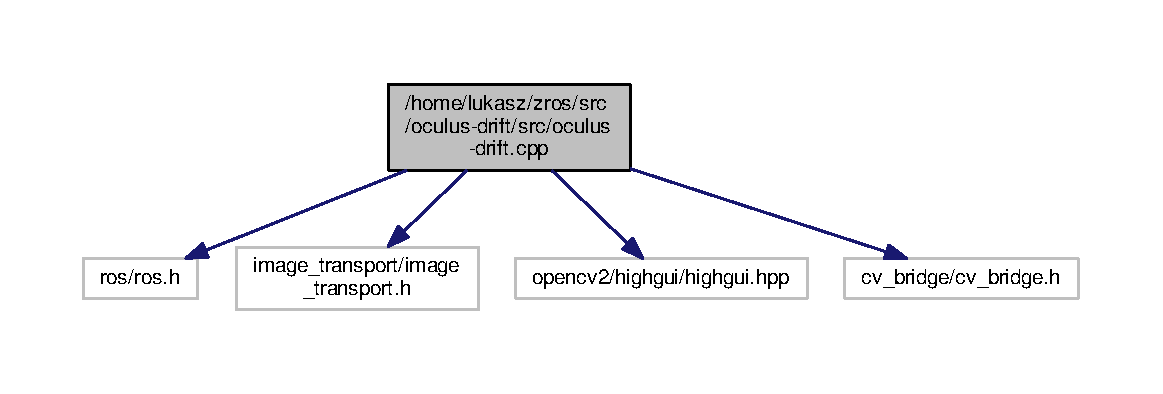
\includegraphics[width=350pt]{oculus-drift_8cpp__incl}
\end{center}
\end{figure}
\subsection*{Functions}
\begin{DoxyCompactItemize}
\item 
void \hyperlink{oculus-drift_8cpp_accfc2045f699b2d8782deca8e1d971cf}{image\+Left\+Callback} (const sensor\+\_\+msgs\+::\+Image\+Const\+Ptr \&msg)
\item 
void \hyperlink{oculus-drift_8cpp_a2bee7d800dfae62103d7aaa2e0961787}{image\+Right\+Callback} (const sensor\+\_\+msgs\+::\+Image\+Const\+Ptr \&msg)
\item 
int \hyperlink{oculus-drift_8cpp_a3c04138a5bfe5d72780bb7e82a18e627}{main} (int argc, char $\ast$$\ast$argv)
\end{DoxyCompactItemize}
\subsection*{Variables}
\begin{DoxyCompactItemize}
\item 
image\+\_\+transport\+::\+Publisher \hyperlink{oculus-drift_8cpp_a1d96cf0c556aa6b5ba7b3b7ad43ca252}{pub\+\_\+left}
\item 
image\+\_\+transport\+::\+Publisher \hyperlink{oculus-drift_8cpp_a69feb6a1df472e1ccf35b35d4f63edd2}{pub\+\_\+right}
\end{DoxyCompactItemize}


\subsection{Function Documentation}
\index{oculus-\/drift.\+cpp@{oculus-\/drift.\+cpp}!image\+Left\+Callback@{image\+Left\+Callback}}
\index{image\+Left\+Callback@{image\+Left\+Callback}!oculus-\/drift.\+cpp@{oculus-\/drift.\+cpp}}
\subsubsection[{\texorpdfstring{image\+Left\+Callback(const sensor\+\_\+msgs\+::\+Image\+Const\+Ptr \&msg)}{imageLeftCallback(const sensor_msgs::ImageConstPtr &msg)}}]{\setlength{\rightskip}{0pt plus 5cm}void image\+Left\+Callback (
\begin{DoxyParamCaption}
\item[{const sensor\+\_\+msgs\+::\+Image\+Const\+Ptr \&}]{msg}
\end{DoxyParamCaption}
)}\hypertarget{oculus-drift_8cpp_accfc2045f699b2d8782deca8e1d971cf}{}\label{oculus-drift_8cpp_accfc2045f699b2d8782deca8e1d971cf}

\begin{DoxyCode}
10 \{
11   \hyperlink{oculus-drift_8cpp_a1d96cf0c556aa6b5ba7b3b7ad43ca252}{pub\_left}.publish(msg);
12 \}
\end{DoxyCode}
\index{oculus-\/drift.\+cpp@{oculus-\/drift.\+cpp}!image\+Right\+Callback@{image\+Right\+Callback}}
\index{image\+Right\+Callback@{image\+Right\+Callback}!oculus-\/drift.\+cpp@{oculus-\/drift.\+cpp}}
\subsubsection[{\texorpdfstring{image\+Right\+Callback(const sensor\+\_\+msgs\+::\+Image\+Const\+Ptr \&msg)}{imageRightCallback(const sensor_msgs::ImageConstPtr &msg)}}]{\setlength{\rightskip}{0pt plus 5cm}void image\+Right\+Callback (
\begin{DoxyParamCaption}
\item[{const sensor\+\_\+msgs\+::\+Image\+Const\+Ptr \&}]{msg}
\end{DoxyParamCaption}
)}\hypertarget{oculus-drift_8cpp_a2bee7d800dfae62103d7aaa2e0961787}{}\label{oculus-drift_8cpp_a2bee7d800dfae62103d7aaa2e0961787}

\begin{DoxyCode}
15 \{
16   \hyperlink{oculus-drift_8cpp_a69feb6a1df472e1ccf35b35d4f63edd2}{pub\_right}.publish(msg);
17 \}
\end{DoxyCode}
\index{oculus-\/drift.\+cpp@{oculus-\/drift.\+cpp}!main@{main}}
\index{main@{main}!oculus-\/drift.\+cpp@{oculus-\/drift.\+cpp}}
\subsubsection[{\texorpdfstring{main(int argc, char $\ast$$\ast$argv)}{main(int argc, char **argv)}}]{\setlength{\rightskip}{0pt plus 5cm}int main (
\begin{DoxyParamCaption}
\item[{int}]{argc, }
\item[{char $\ast$$\ast$}]{argv}
\end{DoxyParamCaption}
)}\hypertarget{oculus-drift_8cpp_a3c04138a5bfe5d72780bb7e82a18e627}{}\label{oculus-drift_8cpp_a3c04138a5bfe5d72780bb7e82a18e627}

\begin{DoxyCode}
22 \{
23   ros::init(argc, argv, \textcolor{stringliteral}{"oculus\_drift"});
24   ros::NodeHandle nh;
25   image\_transport::ImageTransport it(nh);
26   \hyperlink{oculus-drift_8cpp_a1d96cf0c556aa6b5ba7b3b7ad43ca252}{pub\_left} = it.advertise(\textcolor{stringliteral}{"left/image\_raw"}, 1);
27   \hyperlink{oculus-drift_8cpp_a69feb6a1df472e1ccf35b35d4f63edd2}{pub\_right} = it.advertise(\textcolor{stringliteral}{"right/image\_raw"}, 1);
28   image\_transport::Subscriber sub\_left = it.subscribe(\textcolor{stringliteral}{"/firefly/vi\_sensor/left/image\_raw"}, 1, 
      \hyperlink{oculus-drift_8cpp_accfc2045f699b2d8782deca8e1d971cf}{imageLeftCallback});
29   image\_transport::Subscriber sub\_right = it.subscribe(\textcolor{stringliteral}{"/firefly/vi\_sensor/right/image\_raw"}, 1, 
      \hyperlink{oculus-drift_8cpp_a2bee7d800dfae62103d7aaa2e0961787}{imageRightCallback});
30   cv::Mat image = cv::imread(argv[1], CV\_LOAD\_IMAGE\_COLOR);
31   cv::waitKey(30);
32 
33   ros::Rate loop\_rate(5);
34   \textcolor{keywordflow}{while} (nh.ok()) \{
35 
36     ros::spinOnce();
37     loop\_rate.sleep();
38   \}
39 \}
\end{DoxyCode}


\subsection{Variable Documentation}
\index{oculus-\/drift.\+cpp@{oculus-\/drift.\+cpp}!pub\+\_\+left@{pub\+\_\+left}}
\index{pub\+\_\+left@{pub\+\_\+left}!oculus-\/drift.\+cpp@{oculus-\/drift.\+cpp}}
\subsubsection[{\texorpdfstring{pub\+\_\+left}{pub_left}}]{\setlength{\rightskip}{0pt plus 5cm}image\+\_\+transport\+::\+Publisher pub\+\_\+left}\hypertarget{oculus-drift_8cpp_a1d96cf0c556aa6b5ba7b3b7ad43ca252}{}\label{oculus-drift_8cpp_a1d96cf0c556aa6b5ba7b3b7ad43ca252}
\index{oculus-\/drift.\+cpp@{oculus-\/drift.\+cpp}!pub\+\_\+right@{pub\+\_\+right}}
\index{pub\+\_\+right@{pub\+\_\+right}!oculus-\/drift.\+cpp@{oculus-\/drift.\+cpp}}
\subsubsection[{\texorpdfstring{pub\+\_\+right}{pub_right}}]{\setlength{\rightskip}{0pt plus 5cm}image\+\_\+transport\+::\+Publisher pub\+\_\+right}\hypertarget{oculus-drift_8cpp_a69feb6a1df472e1ccf35b35d4f63edd2}{}\label{oculus-drift_8cpp_a69feb6a1df472e1ccf35b35d4f63edd2}

%--- End generated contents ---

% Index
\backmatter
\newpage
\phantomsection
\clearemptydoublepage
\addcontentsline{toc}{chapter}{Index}
\printindex

\end{document}
